
%!TEX ROOT=main.tex


\part{Hardware}
\label{chap:hw}
%\section{Indroduction}
%\label{sec:hw_intro}


\section{Chassis and transmitter}
\label{sec:hw_base}
\subsection{Background}
The whole project is built on an old entry-level onroad 1/10 chassis from the \textit{Tamiya Quick Drive} series released on Jul 16, 2003 \cite{tamiya}. The RC car was obtained as a childhood gift. It was pre-assembled and came with a 2-channel transmitter communicating at a frequency of \SI{27}{\MHz}. Later the servo broke, and no repair or upgrade parts were available. Since the repair was nearly impossible, but the rest of the chassis was fully functional, it was the perfect choice for a complete rebuild.

The car featured a sealed gearbox, servo, "280" size brushed motor and \SI{9.6}{\V} Ni-Cd battery pack. Due to the age of the product, not much technical information can be found.

\subsection{Modifications}
\label{sub:hw_mods}
All the electronics were removed, leaving only the plastic chassis. The broken 5-wire servo was replaced with a "standard" size hobby servo used in most 1/10 RC cars. The old brushed motor was still functional, but it was decided to replace it with a newer and more powerful one. The only constraint was a shaft size, as the old pinion had to be transferred to the new motor to maintain functionality. Therefore a "2435" size BLDC motor with a \SI{25}{\A} ESC was selected. More information about the servo and BLDC is in sections \ref{sec:hw_servo} and \ref{sec:hw_bldc}. Furthermore, the plastic bearings were replaced by metal ball bearings.

A 2-cell LiPo battery with a capacity of \SI{2200}{\milli\A\hour} was chosen to supply power to the electronics. According to the product specification, this battery should withstand 35C of continuous current \cite{lipo_car}. The term "35C" means "35 times the battery capacity". For this particular battery, that means $35 \cdot \SI{2.2}{\A} = \SI{77}{\A}$ of current, which is more than sufficient.

The transmitter underwent a similar procedure. The original circuit board and the antenna were also removed, retaining only trigger potentiometers and plastic parts. Potentiometers used for throttle and steering trimming were replaced with rotary encoders. Again, the power supply is a 2-cell LiPo battery with a lower capacity of only \SI{900}{\milli\A\hour} and 25C of continuous current \cite{lipo_tx}.



\section{Servo}
\label{sec:hw_servo}
A servomotor, or servo for short, is an actuator used for precise output shaft positioning. It consists of a motor with position feedback and a control board. RC servos are controlled using a 50Hz PWM signal. The output angle is linearly dependent on a pulse width between \SI{1}{\ms} and \SI{2}{\ms}. The diagram in figure \ref{fig:servo_control} illustrates typical timing.
\begin{figure}[t]
\centering
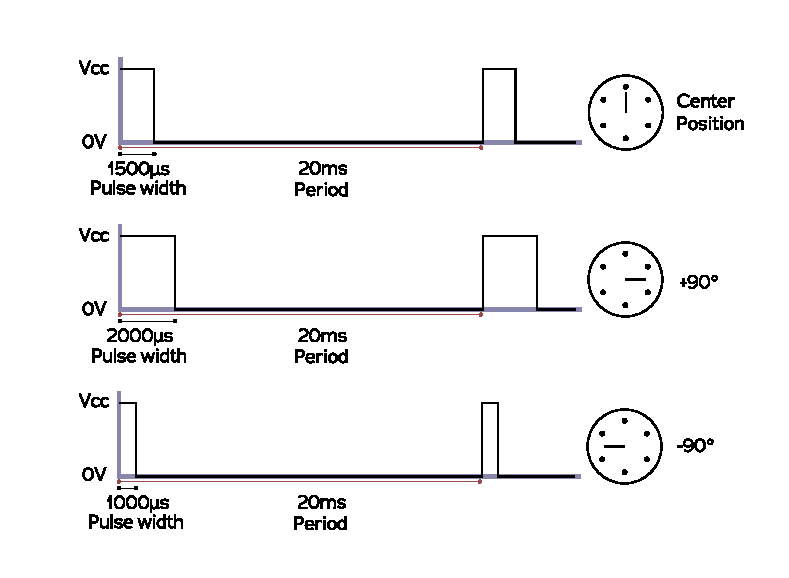
\includegraphics[width=0.7\linewidth]{fig/Servomotor_Timing_Diagram.pdf}
\caption{Servomotor timing diagram \cite{servo_control}}
\label{fig:servo_control}
\end{figure}

The servo used in the car is \textit{TowerPro} MG995. It has metal gears and operating voltage between \SI{4.8}{\V} to \SI{6.6}{\V}. Speed and torque depend on the supply voltage. According to the product specifications \cite{mg995}, the servo can achieve operating speed of $0.2\, \text{s}/60^\circ$ and torque of \SI{9.4}{\kg\per\cm} with the \SI{4.8}{\V} supply voltage. From the operating speed we can calculate angular velocity: 
\begin{equation}
\omega = \frac{d \theta}{d t} = \frac{\frac{\pi}{3}}{0.2} \doteq 5.236\ \unit{\radian\per\second}\ ,
\end{equation}
where $\frac{\pi}{3}$ is $60^\circ$ converted to radians.
Since the servo supply voltage is \SI{5}{\V}, both speed and torque values should be slightly higher.


\section{Motor and ESC}
\label{sec:hw_bldc}
As mentioned in section \ref{sub:hw_mods}, the biggest BLDC with a shaft diameter of \SI{2}{\mm} was selected to replace the old brushed one. The motor was supplied in a set including a \SI{25}{\A} Electronic Speed Controller (ESC). The type is \textit{GoolRC} 2435 \SI{4800}{\Kv}\footnote{\unit{Kv} refers to rpm/V with no load attached to the motor shaft.} BLDC; available information about the motor is in table \ref{tab:BLDC_spec} and about ESC in table \ref{tab:ESC_spec}.

Originally the brass pinion was press-fitted to the motor; however, the shaft began to slip inside the pinion. Therefore it was soldered to the shaft with the help of solder paste and a hot-air station.

Since the BLDC motor is directly connected to the ESC and the control board communicates only with the ESC, the BLDC is considered a black box.

RC ESCs are controlled the same way as RC servos; thus, the same timing diagram in figure \ref{fig:servo_control} applies. The only difference is the resulting motion. Pulse width with a duration of \SI{2}{\ms} equals full forward acceleration, pulse width with a duration of \SI{1.5}{\ms} equals neutral, and pulse width with a duration of \SI{1}{\ms} equals full brake/reverse.

Whether the brake or reverse is activated depends on the actual motion of the motor. If the car is going forward (meaning the motor rotates forward) and the pulse width becomes lower than \SI{1.5}{\ms}, first, the brake is activated and remains activated until the pulse width is again \SI{1.5}{\ms} or greater. The car must be almost static to start reversing; otherwise, the ESC will stay in brake mode. If the car is static or is already reversing, a pulse width lower than \SI{1.5}{\ms} activates reverse mode.

\begin{table}[t]
   %\renewcommand{\arraystretch}{1.1}
   \tabcolsep 18pt
   \centering
    \caption{BLDC specifications}\label{tab:BLDC_spec}   
    \begin{tabular}{l r}
       \noalign{\hrule height 1.1pt}\noalign{\smallskip}	   
	Power			& 300\unit{\W}\\
	Max. voltage   	& 12.6\unit{\V}\\
	Max. current   	& 24\unit{\A}\\
	Rotor poles	   	& 4 \\
	\unit{\Kv} rating	  	& 4800 \\
	Length			& 24\unit{\mm} \\
	Diameter			& 35\unit{\mm} \\
	Shaft diameter	& 2\unit{\mm} \\
       \noalign{\smallskip}\noalign{\hrule height 1.1pt}
    \end{tabular}
\end{table} 
\begin{table}[t]
   %\renewcommand{\arraystretch}{1.1}
   \tabcolsep 12pt
   \centering
    \caption{ESC specifications}\label{tab:ESC_spec} 
    \begin{tabular}{l r}
       \noalign{\hrule height 1.1pt}\noalign{\smallskip}
	Continuous current		& 25\unit{\A}\\
	Instantaneous current   	& 50\unit{\A}\\
	BEC type				   	& 5\unit{\V}, 2\unit{\A}\\
	Battery				   	& 2-3 Cell LiPo \\
       \noalign{\smallskip}\noalign{\hrule height 1.1pt}
    \end{tabular}
\end{table} 

\section{Control board}
\label{sec:hw_control}
Prototyping was mainly done on the breadboard using the \textit{RobotDyn's} BlackPill development board featuring STM32F303CCT6 microcontroller \cite{black_pill}. The board uses a similar size and form factor as the popular BluePill board equipped with STM32F103C8T6 \cite{blue_pill}. Both these boards were readily available.

BlackPill was selected for its better processor based on an ARM M4 core with FPU, larger memories, and more advanced peripherals. Thus, it is more suitable for processing data from more sensors, especially when using floating point arithmetics. The board is shown in figure \ref{fig:black_pill}.
\begin{figure}[t]
\centering
\includegraphics[width=0.5\linewidth]{fig/placeholder.jpg}
\caption{*PLACEHOLDER* RobotDyn BlackPill development board}
\label{fig:black_pill}
\end{figure}


\section{Communication}
\label{sec:hw_comm}
The project uses wireless modules equipped with nRF24L01+ transceiver chip from \textit{Nordic Semiconductor} [\todo citace], a power amplifier, a low-noise amplifier, and an external antenna. The chip operates in the worldwide \SI{2.4}{\GHz} ISM band and communicates with the MCU using the SPI bus. Configurable parameters include channel, data rate, and output power. These modules fit all the requirements, and in addition, they are cheap and readily available.

According to the product specification [\todo cit-Amazon], the range should be more than \SI{800}{\m} line-of-sight. Thanks to the \textit{Enhanced ShockBurst protocol} and its Auto Acknowledgement function [\todo citace], attaching a small payload to the ACK packet is possible. This feature is advantageously used to report car status back to the transmitter.

An additional adapter board is utilized to supply voltage to the nRF24 module. It has the same pinout and includes a voltage regulator with all needed external components. The Adapter board is powered with \SI{5}{\V}, which are then regulated to \SI{3.3}{\V}. This setup ensures a stable power supply for the nRF24 module.

As the adapter board is only equipped with a pin socket for connection, which is unsuitable for use in vibration generating environments, it was removed. The nRF24 module was instead soldered directly to the adapter, as were the wires. The entire communication module is thus more robust and takes up less space.


\section{Sensors}
\label{hw_sensors}
In addition to measuring the voltage, which is necessary for battery monitoring and is realized using a voltage divider, the car also measures current and BLDC case temperature. It is also equipped with 6-axis IMU. In the project's present state, data from sensors are mainly informative and are not used for control purposes.

The transmitter does not use any particular sensor; only battery voltage is measured via the voltage divider.

\subsection{Current}		%TODO obrazek?
The current is measured using a module with a 30A version of an ACS712 chip from \textit{Allegro MicroSystems}. It is a small linear current sensor based on the Hall effect. Current flowing through the sensor's copper terminals generates a magnetic field, which is then sensed by the integrated Hall-effect circuit.

The output of the sensor is a voltage proportional to the flowing current. If no current is flowing, the sensor output is the supply voltage divided by two. If a positive current flows, the output voltage increases, whereas the output voltage decreases if the current is negative.

Current sense terminals are electrically isolated from the rest of the sensor; therefore, it is possible to measure high voltages without external electrical isolation. The sensor is capable of measuring both AC and DC current with a stated total output error of $1.5\%$ \cite{acs_datasheet}. 

\subsection{Temperature}	%TODO obrazek?
A digital thermometer DS18B20 provides temperature measurement. The sensor is manufactured by \textit{Dallas Semiconductor}, which \textit{Maxim Integrated} later acquired. It can measure temperatures from \SI{-55}{\degreeCelsius} to \SI{125}{\degreeCelsius}. It has a programmable resolution ranging from 9 to 12 bit and $\pm$\SI{0.5}{\degreeCelsius} over most of the measuring range. The sensor uses a 1-Wire interface, which requires only one pin for communication. When combined with parasitic power mode, the whole thermometer requires only two pins for operation \cite{ds_datasheet}.

The project uses the TO-92 package, which was advantageous because of the limited space around the BLDC. The small size made it possible to mount the sensor on the back of the motor housing with the aid of heat-conducting foil.

\subsection{IMU}			%TODO obrazek?
For motion measurements, a module with MPU6050 from \textit{InvenSense} was selected as it was the cheapest option. The sensor packs a 3-axis accelerometer, which provides linear acceleration data, and a 3-axis gyroscope, which provides angular velocity data, in one chip. Both the accelerometer and gyroscope have programmable measurement ranges. Communication with the sensor is performed using the I\textsuperscript{2}C bus. An external 3-axis magnetometer can be attached straight to the sensor, extending the sensor's capability \cite{mpu_datasheet}.

The sensor claims it has a DMP (Digital Motion Processor) capable of merging the accelerometer and gyroscope data on-chip. Sadly, this feature is undocumented and available only when using \textit{InvenSense's} official \textit{Embedded MotionApps software}. Another possibility would be using \textit{I\textsuperscript{2}Cdevlib}, where the DMP functionality was reverse-engineered \cite{i2cdevlib}. However, the \textit{I\textsuperscript{2}Cdevlib} is written for Arduino and would require porting the code to the STM32 with uncertain results. Therefore only raw accelerometer and gyroscope data are used.

\section{Status info}
\label{sec:hw_status}
Neither the RC car nor the transmitter reported any status in the original version. The user had to check the battery state himself; otherwise, the battery could be discharged entirely and damaged. Since LiPo batteries should not be discharged below a certain threshold, the usual rule of thumb across the RC community is not to discharge the battery below \SI{3.1}{\V} per cell, it was necessary to report the battery status.

An RGB LED was chosen for that purpose because it is possible to quickly report the various states to the user using different colors. On the other hand, it is unsuitable for visualizing values such as temperature. Besides, the transmitter has its own battery, whose status should also be reported to the user, and that would need 2 LEDs. The single RGB LED was therefore insufficient for the transmitter.

For this reason, the display seemed like a good alternative and replacement. An OLED display was convenient as its power consumption is low, it is readable in direct sunlight, and thanks to only one color, it is fast. The disadvantage is its small size, which complicates the orientation in the displayed data.

Considering all the factors, both the RGB LED and the OLED display were used. RGB LED serves as a fast state notifier, and further status information can be found on the display.

Both car and transmitter use RGB LED with a common anode and monochrome OLED display module with SSD1306 chip communicating using I\textsuperscript{2}C bus [\todo citace].


%\begin{table}[t]
%\centering
%\caption{*PLACEHOLDER* BLDC specifications} %TODO citace
%\includegraphics[width=0.8\linewidth]{support/pic/placeholder.jpg}
%\label{tab:BLDC_spec}
%\end{table}

